\documentclass[a4paper, 12pt]{article}%тип документа

%отступы
\usepackage[left=2cm,right=2cm,top=2cm,bottom=3cm,bindingoffset=0cm]{geometry}

%Русский язык
\usepackage[T2A]{fontenc} %кодировка
\usepackage[utf8]{inputenc} %кодировка исходного кода
\usepackage[english,russian]{babel} %локализация и переносы

%Вставка картинок
\usepackage{wrapfig}
\usepackage{graphicx}
\graphicspath{{pictures/}}
\DeclareGraphicsExtensions{.pdf,.png,.jpg}

%оглавление
\usepackage{titlesec}
\titlespacing{\chapter}{0pt}{-30pt}{12pt}
\titlespacing{\section}{\parindent}{5mm}{5mm}
\titlespacing{\subsection}{\parindent}{5mm}{5mm}
\usepackage{setspace}

%Графики
\usepackage{multirow}
\usepackage{pgfplots}
\pgfplotsset{compat=1.9}

%Математика
\usepackage{amsmath, amsfonts, amssymb, amsthm, mathtools}

%Стиль страницы
\usepackage{fancyhdr}
\pagestyle{fancy}

\begin{document}

\begin{titlepage}

\begin{center}
%\vspace*{1cm}
\large\textbf{Московский Физико-Технический Институт}\\
\large\textbf{(государственный университет)}
\vfill
\line(1,0){430}\\[1mm]
\huge\textbf{Работа 3.6.1}\\
\line(1,0){430}\\[1mm]
\vfill
\large Сибгатуллин Булат, ФРКТ\\
\end{center}

\end{titlepage}
\fancyhead[L] {Работа 3.6.1}
\noindent \textbf{Цель работы: изучить спектральный состав периодических сигналов.} \\
\indent text\\
\noindent \textbf{В работе используются: анализатор спектраб генератор прямоугольных импульсов и сигналов специальной формы, осциллограф.} \\
\indent text

\section*{Описание работы}

В работе изучается спектральный состав периодических электрических сигналов различной формы: последовательность прямоугольных импульсов, последовательности цугов и амплитудно-модулированных колебаний. Спектры этих сигналлов наблюдаются с помощью анализатора спектра и сравниваются с рассчитанными теоретически.

Периодическая функция может быть представлена в виде бесконечного ряда гармонических функций - ряда Фурье:

\[f(t) = \sum\limits_{n = -\inf}^{\inf} c_n e^{in\omega_0 t} \quad \text{или} \quad 
f = \sum\limits_{n = 0}^{\inf} a_n \cos (n \omega_0 t + \phi_n ).\]

Здесь $\omega_0 = 2\pi /T$, где $T$ - период функции $f(t)$. Коэффициенты ${c_n}$ могут быть найдены по формулы:

\[c_n = \frac{1}{T} \int\limits_0^T f(t) e^{-in \omega_0 t} dt.\]

Наборы коэффициентов разложения в комплексной ${c_n}$ и действительной ${a_n, \phi_n}$ формах связаны соотношением:

\[a_n = 2 | c_n |, \quad \phi_n = \text{arg}c_n.\]

В качестве простейшего спектрального анализатора можно использовать высокодобротный колебательный контур с подстраиваемой ёмкостью или индуктивностью. Такой контур усиливает те гармоники входного сигнала $f(t)$, частота которых близка к резонансной $\nu_0 = 1/(2\pi \sqrt{LC}$ и практически не реагируют на частоты, далёкие от $\nu_0$. С точки зрения преобразования гармоник колебательный контур является узкополосным фильтром с шириной полосу пропускания порядка $\bigtriangleup \sim \nu_0/Q,$ где $Q = \frac{1}{R}\sqrt{\frac{L}{C}} \gg 1$ - его добротность. Амплитуда колебаний в контуре пропорциональна амплитуде $|c(\nu_0)|$ гармоники в спектре функции $f(t)$, частота которой совпадает с $\nu_0$. Таким образом, меняя резонансную частоту контура, можнно <<просканировать>> весь спектр входного сигнала.

\section*{Эскпериментальная установка}

\begin{figure}[h!]
\centering
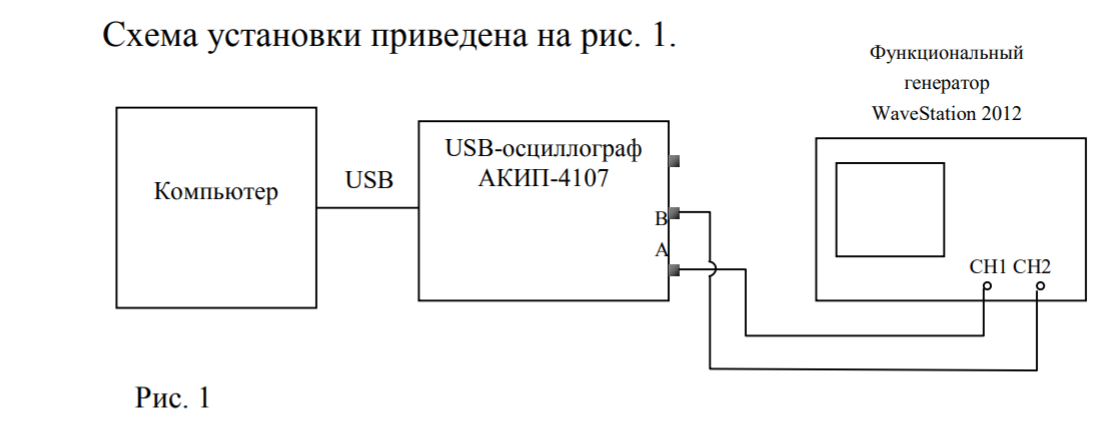
\includegraphics[scale=0.6]{images/scheme.png}
\label{fig:Image1}
\end{figure}

Функциональный генератор WaveStation 2012 позволяет сформировать два
различных электрических сигнала, которые выводятся на два независимых
канала – "CH1" и "CH2". Сигнал с канала "CH1" подается на вход "A", а
сигнал с канала "CH2" – на вход "B" USB-осциллографа. Затем эти сигналы подаются на вход компьютера через USB-соединение. При работе USBосциллографа в режиме осциллографа, на экране компьютера можно
наблюдать каждый из сигналов в отдельности, а также их произведение.
В режиме спектроанализатора можно наблюдать спектры этих сигналов. При включении функционального генератора, на его экране отображается информация о параметрах электрического сигнала.

\end{document}